\chapter{Documento de Diseño del Juego (GDD)}
\label{GDD}
\section{Características}
\begin{itemize}
	\item \textbf{Título:} N/A. \LaTeX \LaTeX \LaTeX \LaTeX
	\item \textbf{Plataforma:} \ac{PC} (Windows y Linux).
	\item \textbf{Género:} \acf{RTS}.
	\item \textbf{Idioma:} Inglés.
	\item \textbf{Clasificación:} PEGI 7\footnote{Web de la asociación https://pegi.info}
\end{itemize}

\section{Descripción general}
El juego que se pretende desarrollar consiste en un \ac{RTS} haciendo hincapie en el
apartado de navegación por el mapa y el combate, dejando así la gestión de recursos
y el desarrollo de una civilización o facción a un lado debido a las limitaciones
de tiempo y personal. A lo largo de los distintos niveles, el jugador deberá hacer
frente a distintos desafios como pueden ser: trasladar todas sus unidades de un punto
del mapa a otro mientras se evita la muerte de algún personaje importante y/o eliminar
a todas las entidades enemigas del escenario.

\section{Mecánicas}
La finalidad del juego es la de completar los distintos niveles de forma satisfactoria,
esto sucederá ya sea cuando eliminemos a todas las unidades enemigas desplegadas a lo
largo del nivel o alcancemos el punto indicado. Como herramienta para alcanzar este
objetivo dispondremos de un ejercito a nuestro mando el cual deberemos gestionar de
forma efectiva para sortear los obstáculos y desafios propuestos.

El jugador será capaz de seleccionar con el ratón las unidades exactas sobre las que
quiere lanzar la acción y seleccionar o deseleccionar todas la unidades a su
disposición mediante atajos de teclado en cualquier momento. Las acciones disponibles
para su uso serán las de desplazar las unidades, hacer que se queden a la espera y
realizar un ataque sobre las unidades rivales que se indiquen. Como puede verse en la
imágen~\ref{fig:unit-selec}

El jugador perderá cuando todas sus unidades mueran.

\begin{figure}[ht]
\centering
\begin{minipage}[c]{0.45\linewidth}
	\hspace{1cm}
	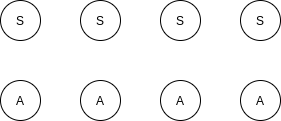
\includegraphics[width=0.7\textwidth]{imagenes/gdd/non-selection.png}
\end{minipage}
\begin{minipage}[c]{0.45\linewidth}
	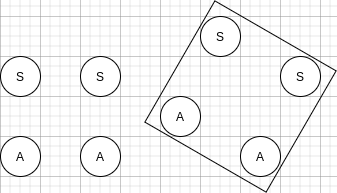
\includegraphics[width=0.7\textwidth]{imagenes/gdd/selection.png}
\end{minipage}	
\caption{MockUp selección.}
\label{fig:unit-selec}
\end{figure}

\section{Unidades}
Entre las unidades podemos encontrar diferentes arquetipos con carácteristicas propias
que nos permitiran crear variedad en las posibles soluciones a la hora de superar el
nivel.

Los distintos tipos son los siguientes:
\begin{itemize}
	\item \textbf{Soldado:} es la unidad más básica que podemos encontrar en el campo de
							guerra, esta armado con una espada y posee estadisticas
							bajas.
	\item \textbf{Arquero:} va equipado con arco y flechas para atacar a distancia a
							sus rivales, tiene menos resistencia que los soldados por
							lo que tendremos que protegerlos para asegurar su
							supervivencia.
\end{itemize}

\section{Controles}
A la hora de jugar tendremos una serie de teclas asignadas a las acciones que el
jugador puede realizar cuando interactúe con el juego. Para enumerarlas dividiremos las
acciones en dos grupos, dependiendo de si son para navegar por los menús o si
representan acciones durante el \textit{gameplay}.

Las teclas para navegar por los menús son las siguientes:

\begin{itemize}
	\item \textbf{Enter:} mediante esta tecla podremos avanzar por los menús una vez estemos sobre la opción deseada.
	\item \textbf{Retroceso:} mediante esta otra podremos ir hacía atrás por los menús.
	\item \textbf{Escape:} esta nos permitirá salir de la ejecución del programa.
\end{itemize}

Las asignadas para jugar son las siguientes:

\begin{itemize}
	\item \textbf{Click derecho:} mediante esta tecla del ratón podremos seleccionar la
	unidad sobre la que queremos trabajar, si mantenemos pulsado y arrastramos por el
	escenario podremos seleccionar varias unidades cercanas. Si no se selecciona ninguna
	unidad, se deshará la selección actual.
	\item \textbf{Click izquierdo:} con esta otra podremos seleccionar donde queremos
	desplazar a las unidades seleccionadas y/o atacar a otras unidades.
	\item \textbf{R:} usaremos esta tecla para deseleccionar todas las unidades desde
	el teclado.
	\item \textbf{T:} la usaremos para seleccionar a todas las unidades,
	independientemente de donde se encuentren.
\end{itemize}

\section{Pantallas}
Al ejecutar el programa la primera pantalla que aparecerá será la de 
inicio~\ref{mockup_ini}. Se compone del título del juego, la fecha de lanzamiento,
el nombre del desarrollador y un mensaje que nos indica que tenemos que pulsar al tecla
\textit{entre} para continuar, esta pantalla se mantendrá hasta que el jugador presione
dicha tecla.

\begin{figure}[ht]
\centering
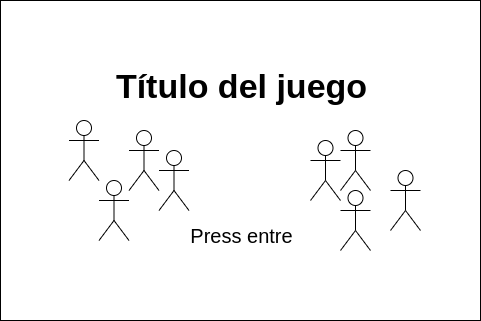
\includegraphics[width=0.45\textwidth]{imagenes/gdd/pantallas/Pantalla_ini.png}
\caption{MockUp pantalla de inicio.}
\label{mockup_ini}
\end{figure}

Una vez pulsado el botón indicado se procederá a cargar el juego mientras se muestra
una barra que indica el progreso de cargado~\ref{mockup_carga}.

\begin{figure}[ht]
\centering
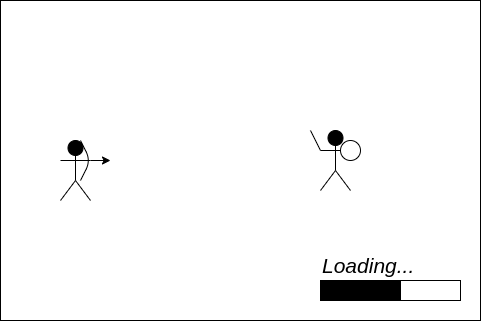
\includegraphics[width=0.45\textwidth]{imagenes/gdd/pantallas/Pantalla_carga.png}
\caption{MockUp pantalla de carga.}
\label{mockup_carga}
\end{figure}

A continuación de la carga pasaremos directamente al escenario donde se desarrollará el
\textit{gameplay} y nos mantendremos en esta pantalla hasta que termine el juego, ya sea
por victoria o derrota del jugador~\ref{mockup_juego}.

\begin{figure}[ht]
\centering
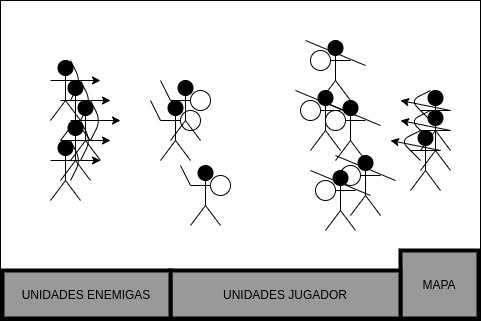
\includegraphics[width=0.45\textwidth]{imagenes/gdd/pantallas/Pantalla_gameplay.png}
\caption{MockUp escenario juego.}
\label{mockup_juego}
\end{figure}

El final de la partida nos trae dos posibles escenarios, la victoria y la derrota. 
Para cada uno saldrá su respectivo mensaje~\ref{mockup_victoria}~\ref{mockup_derrota}
y pasado un momento se nos mandará automáticamente a la pantalla de
inicio~\ref{mockup_ini}.

\begin{figure}[hb]
\centering
\begin{minipage}[c]{0.45\linewidth}
	\hspace{9mm}
	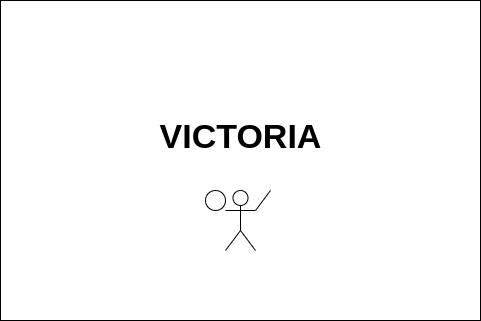
\includegraphics[width=0.7\textwidth]{imagenes/gdd/pantallas/Pantalla_victoria.png}
	\caption{MockUp victoria.}
	\label{mockup_victoria}
\end{minipage}
\begin{minipage}[c]{0.45\linewidth}
	\hspace{9mm}
	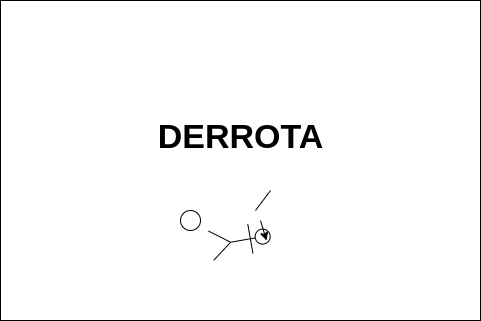
\includegraphics[width=0.7\textwidth]{imagenes/gdd/pantallas/Pantalla_derrota.png}
	\caption{MockUp derrota.}
	\label{mockup_derrota}
\end{minipage}	
\end{figure}

Como última pantalla con la que el jugador podrá interactuar es la del menú de
pausa~\ref{mockup_pausa} en el cual se le dará la opción de salir o de volver a la
partida, mientras esta pantalla este activa la acción en el juego se paralizará hasta
que el jugador decida. 

\begin{figure}[ht]
\centering
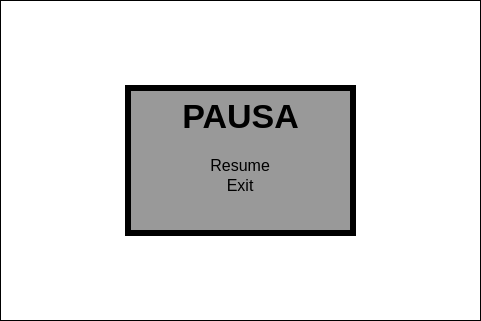
\includegraphics[width=0.45\textwidth]{imagenes/gdd/pantallas/Pantalla_pausa.png}
\caption{MockUp menú de pausa.}
\label{mockup_pausa}
\end{figure}

\section{Estados del juego}

Una vez mostradas todas las posibles pantallas con las que podrá interactuar el jugador
es interesante dibujar un diagrama de flujo que plame sus conexiones y posibilidades
con el fin de crear una representación gráfica que sirva como esquema global.

Dicho esquema podemos encontrarlo en la figura~\ref{esq:flow_juego}.

\begin{figure}[ht]
\centering
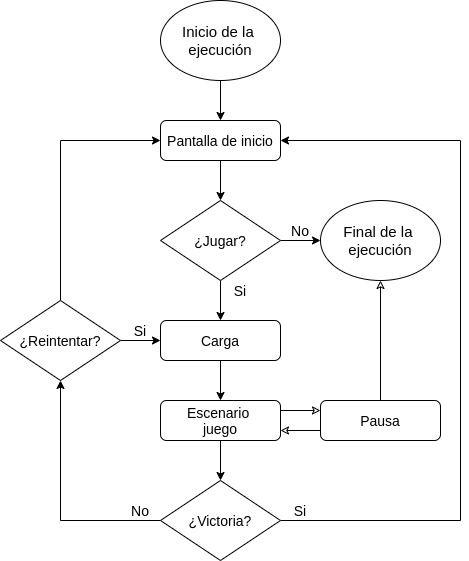
\includegraphics[width=0.45\textwidth]{imagenes/gdd/pantallas/flow_ejecucion.png}
\caption{MockUp escenario juego.}
\label{esq:flow_juego}
\end{figure}

\section{Escenarios}
A lo largo de los niveles la intención es que nos encontremos con distintos biomas como
pueden ser praderas, bosque o desiertos como los que podemos encontrar en \ac{AoE} II
como hemos visto anteriormente en la imágen~\ref{img:aoe_2} o en las
~\ref{img:mapa_aoe1} y ~\ref{img:mapa_aoe2}.

\begin{figure}[ht]
\centering
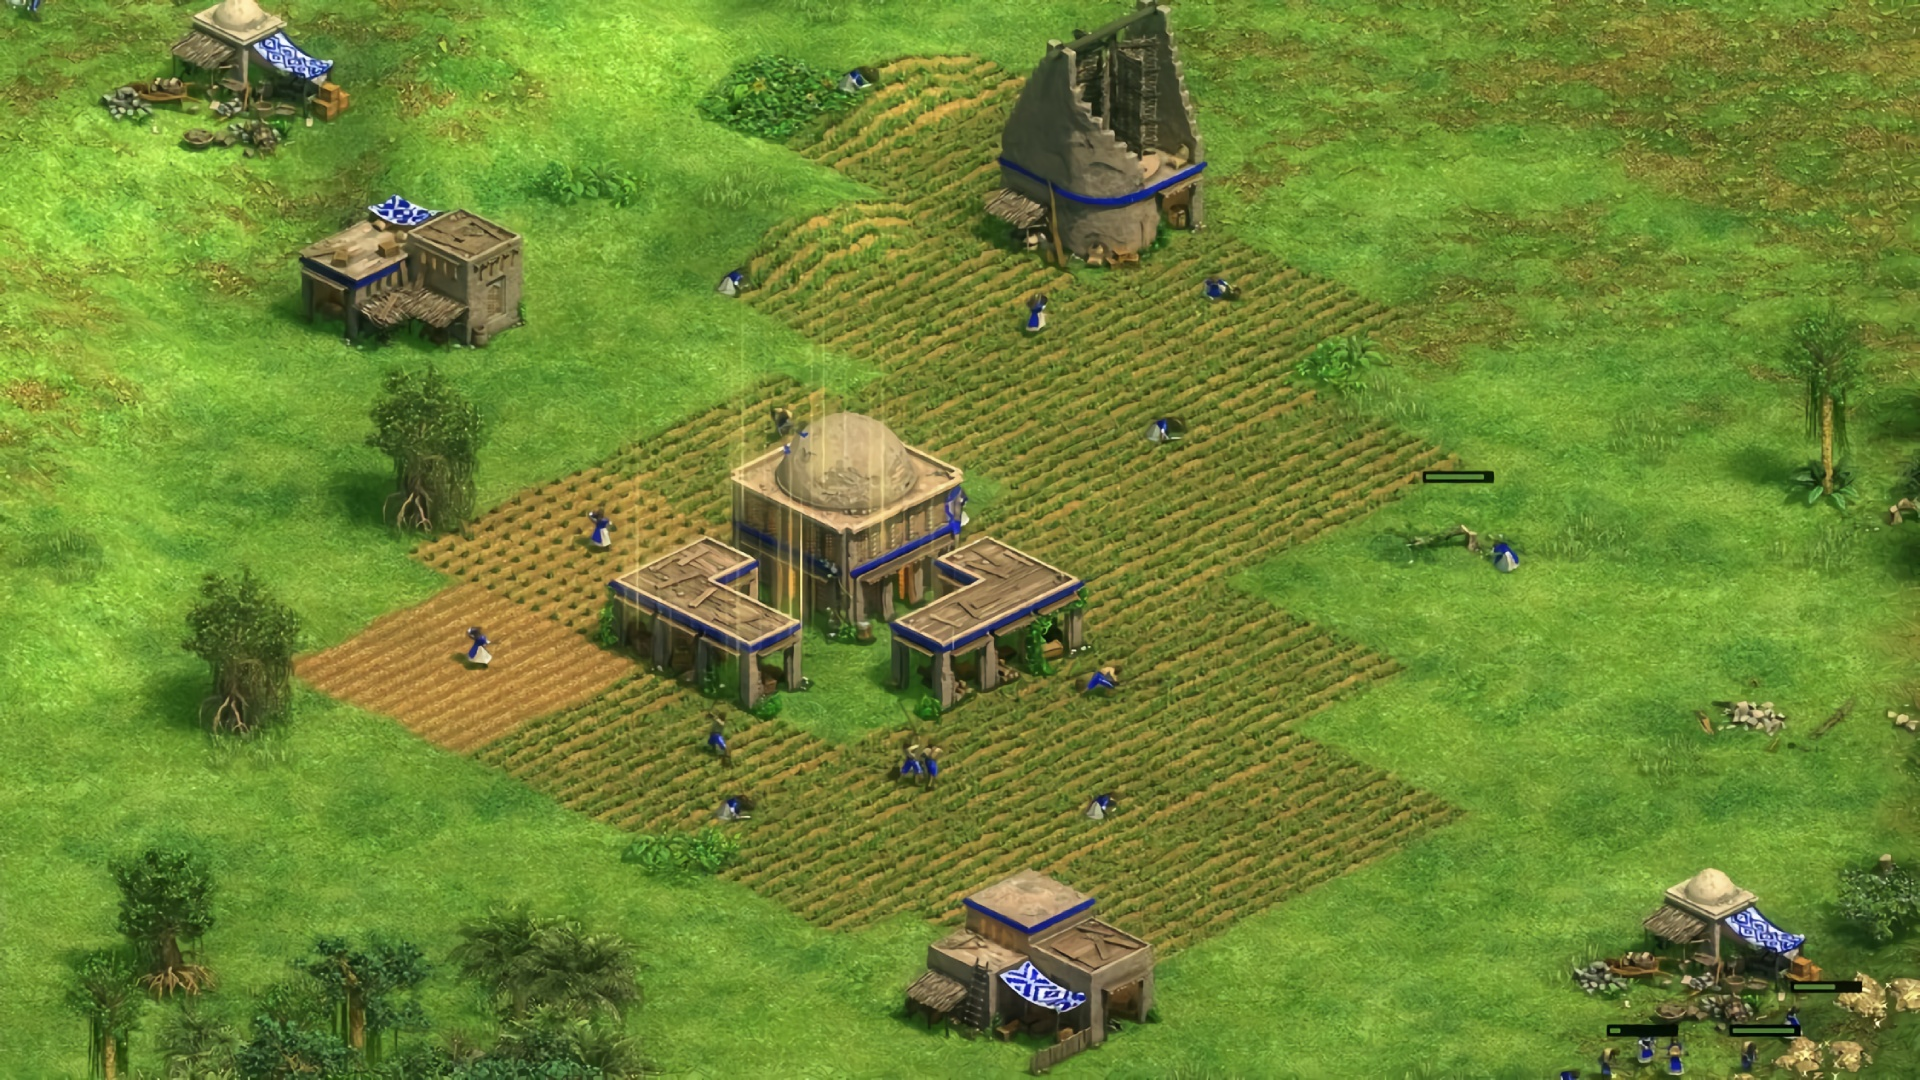
\includegraphics[width=0.6\textwidth]{imagenes/gdd/mapa_aoe_1.jpg}
\caption{Ejemplo escenario con vegetación.}
\label{img:mapa_aoe1}
\end{figure}

\begin{figure}[ht]
\centering
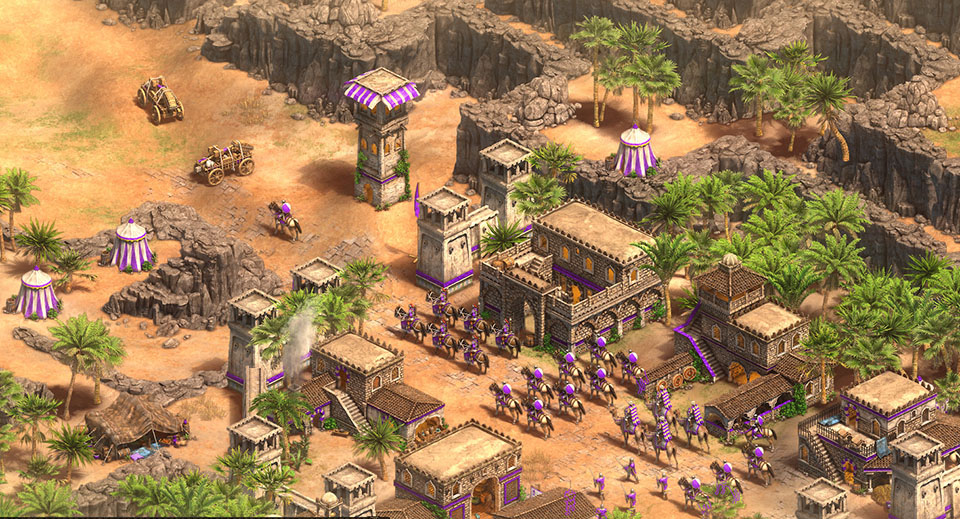
\includegraphics[width=0.6\textwidth]{imagenes/gdd/mapa_aoe_2.jpg}
\caption{Ejemplo escenario desértico.}
\label{img:mapa_aoe2}
\end{figure}

Además de imitar el estilo artístico el juego se desarrollará empleando una cámara
aerea fija manteniendo una perspectiva isométrica que nos permitirá visualizar desde
un punto elevado una gran porción del escenario, esto lo haremos con el fin de dar al
jugador la posibilidad de conocer lo máximo posible el territorio cercano posible y a la
vez le libramos de tener que estar preocuparse de situar la cámara para cada momento. \\
Al mantener una posición fija podemos situar todos los elementos en la escena de forma
que no obstaculicen la visión o molesten al jugador.



